\documentclass[10pt,twocolumn]{article}
\usepackage[margin=1.8 cm]{geometry}
\setlength{\columnsep}{0.7 cm}

\usepackage[]{graphicx}
\usepackage[skip=10pt,font=small]{caption,subcaption}

\usepackage[usenames, dvipsnames]{color}

\usepackage{amsmath}
\usepackage{amssymb}
\usepackage{bm}

\graphicspath{{bbfigs/}}

\begin{document}

\subsection*{Cryogenic temperatures}

As pointed out in the previous subsection, an estimate\footnote{valid for a sufficiently large atom density.} of the time $\tau_c$ until the creation of the first contaminant atom, is \cite{AB}

\begin{displaymath}
\tau_c = \frac{4\delta^2}{\Omega^2}\frac{\tau_0}{b_{nL}N_{\beta}},
\end{displaymath}

\noindent
where $b_{nL}$ is the sum of the branching ratios from the $nL$ Rydberg state\footnote{the one used to dress the ground state.} to the contaminant states that contribute the most to the value of the effective interaction volume $\beta$. $N_{\beta}$ is the number of atoms per volume $\beta$, and $\tau_0$ is the natural lifetime of the  $nL$  state.

The time $\tau_c$ depends on the ambient temperature $T$ through $\tau_0$ and $b_{nL}$. Figures \ref{fig:cthcal1_4} and \ref{fig:cthcal2_4} show this dependence for some $^{87}$Rb $nS$ Rydberg states. These plots were obtained using the estimates from \cite{Beterov2009} and the quasiclassical formulas in \cite{Dyachkov1994}. We also estimated the largest value $T_N^*$ of the temperature $T$ needed to compensate for the avalanche dephasing effect as a function of $N_{\beta}$, see Fig. \ref{fig:cthcal3_4}.

\begin{figure}[]
\begin{minipage}[c][4.5cm][t]{.24\textwidth}
  \vspace*{\fill}
  \centering
  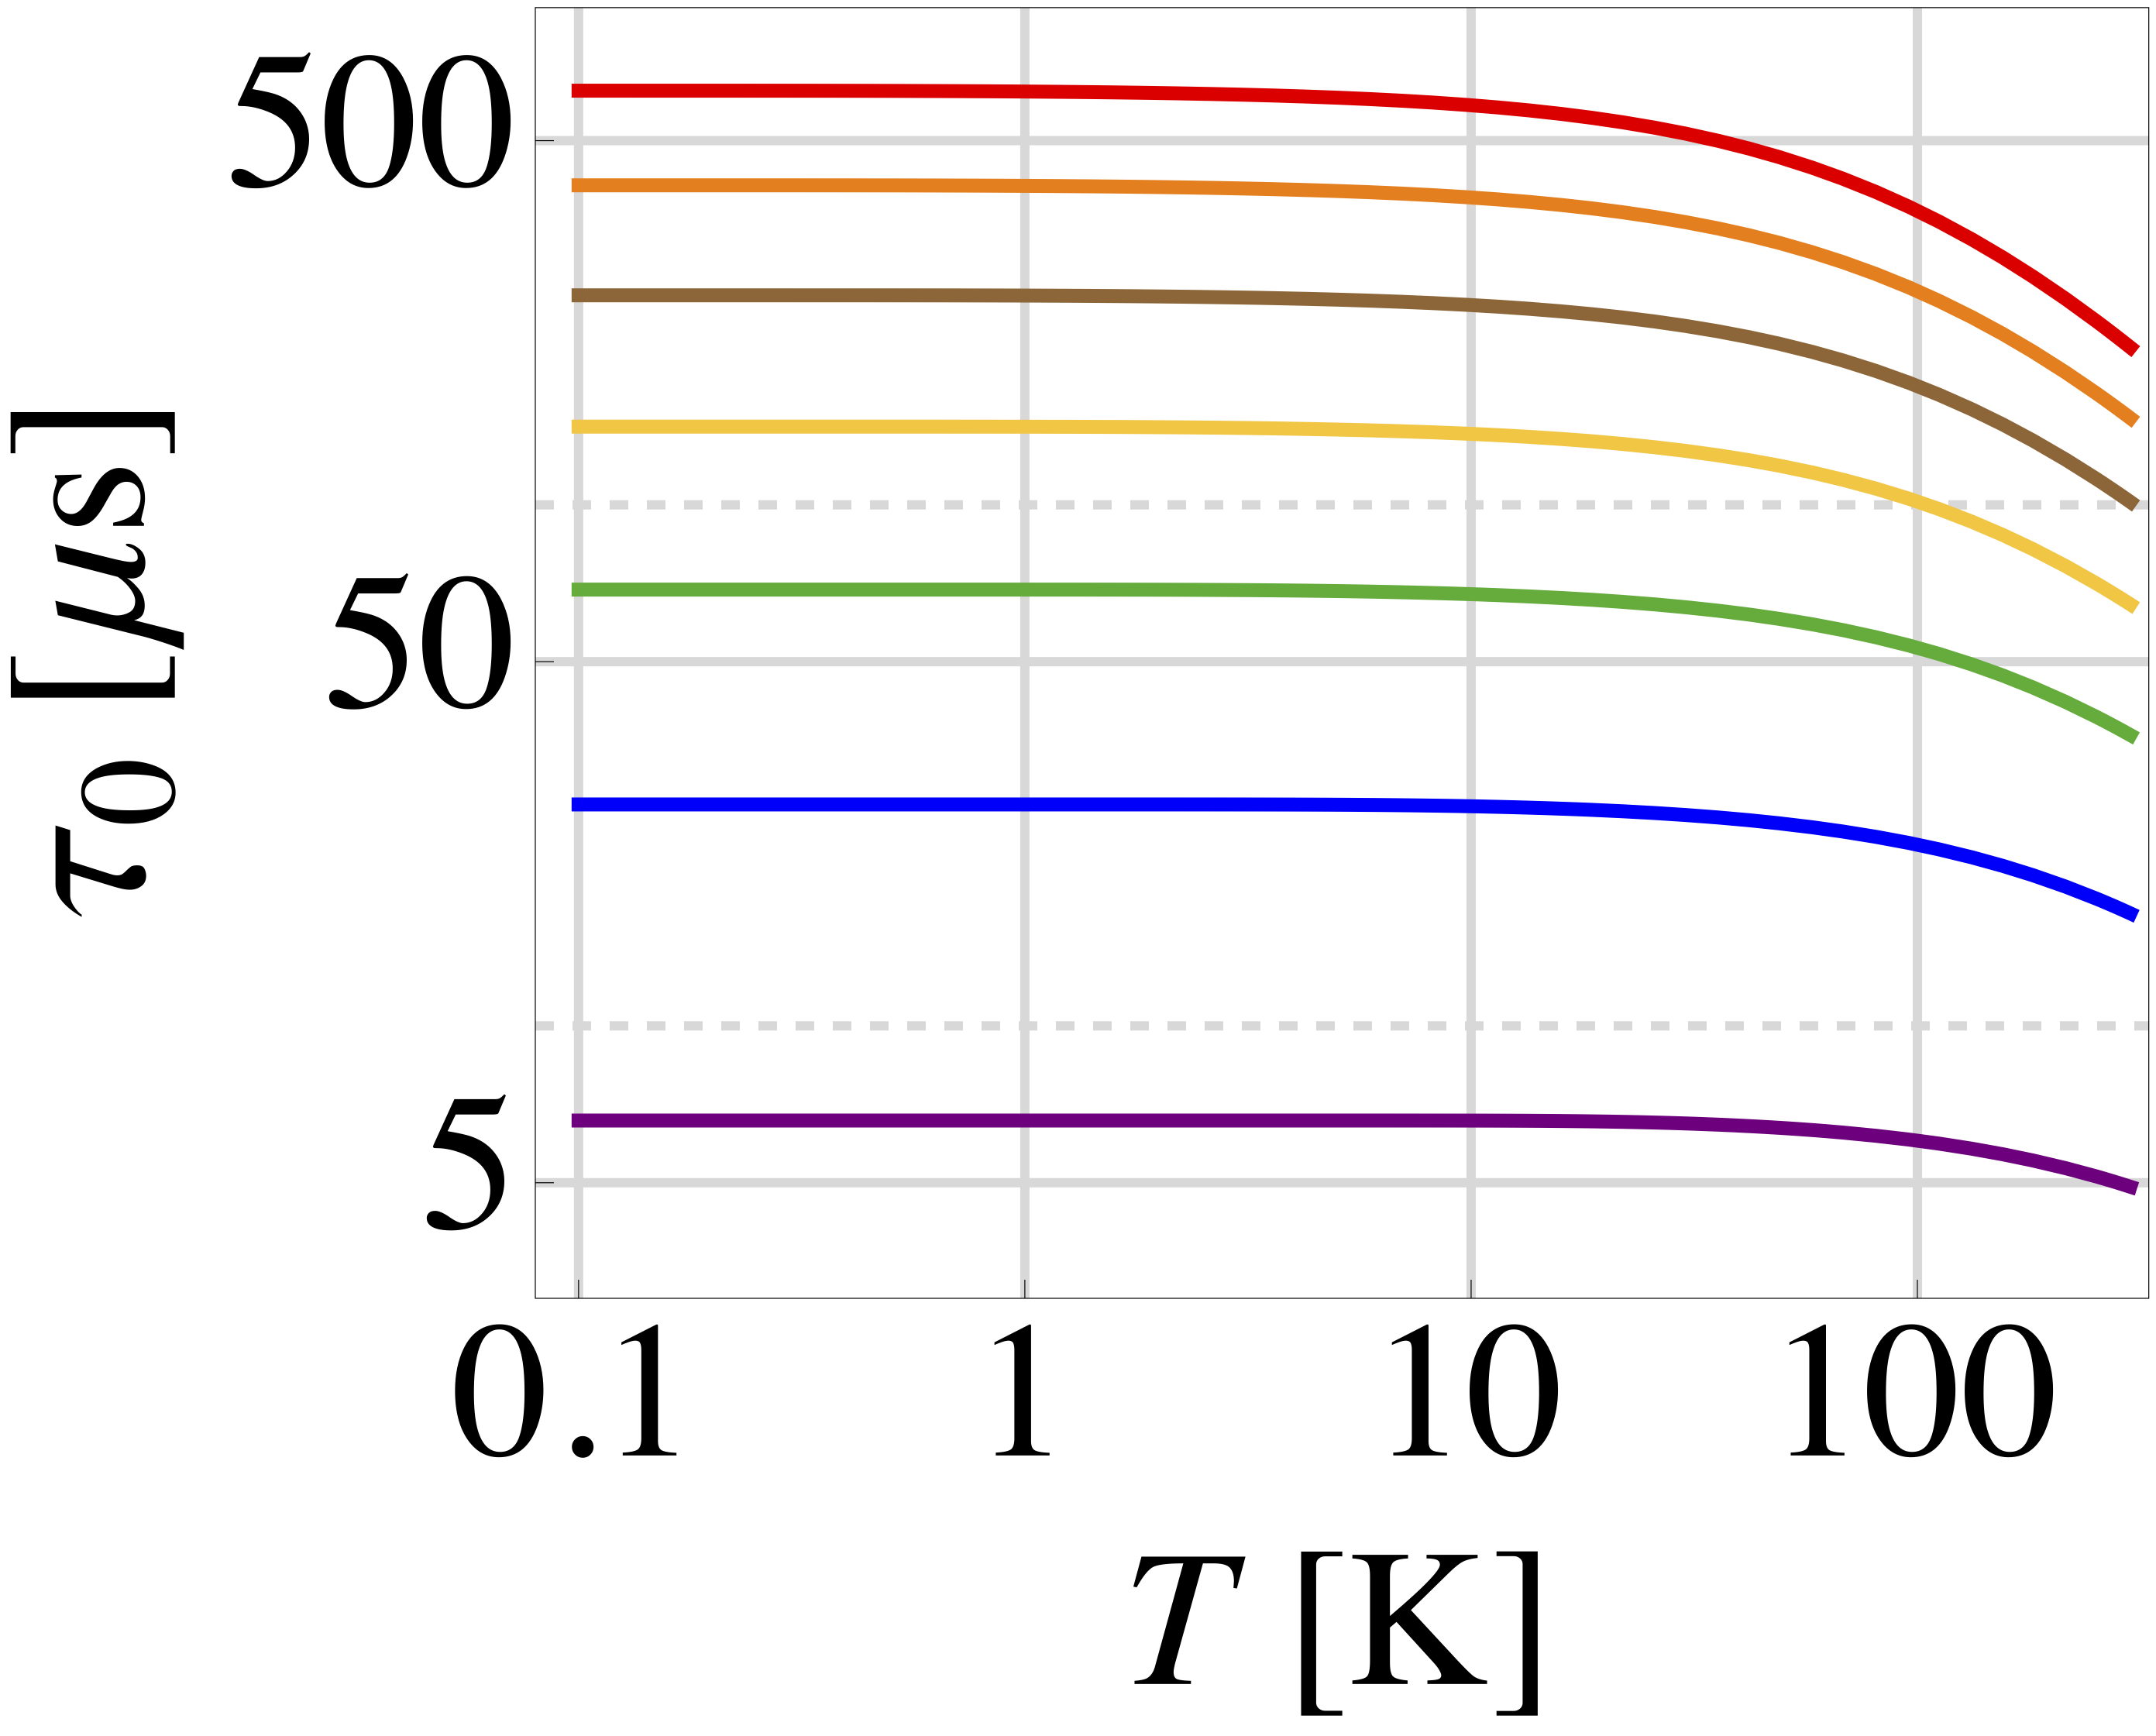
\includegraphics[width=3.8cm,height=3.2cm]{tauloglog.png}
  \subcaption{\iffalse$N^*_T$ vs $T$\fi}
  \label{fig:cthcal1_4}
  %
\end{minipage}%
\begin{minipage}[c][4.5cm][t]{.24\textwidth}
  \vspace*{\fill}
  \centering
  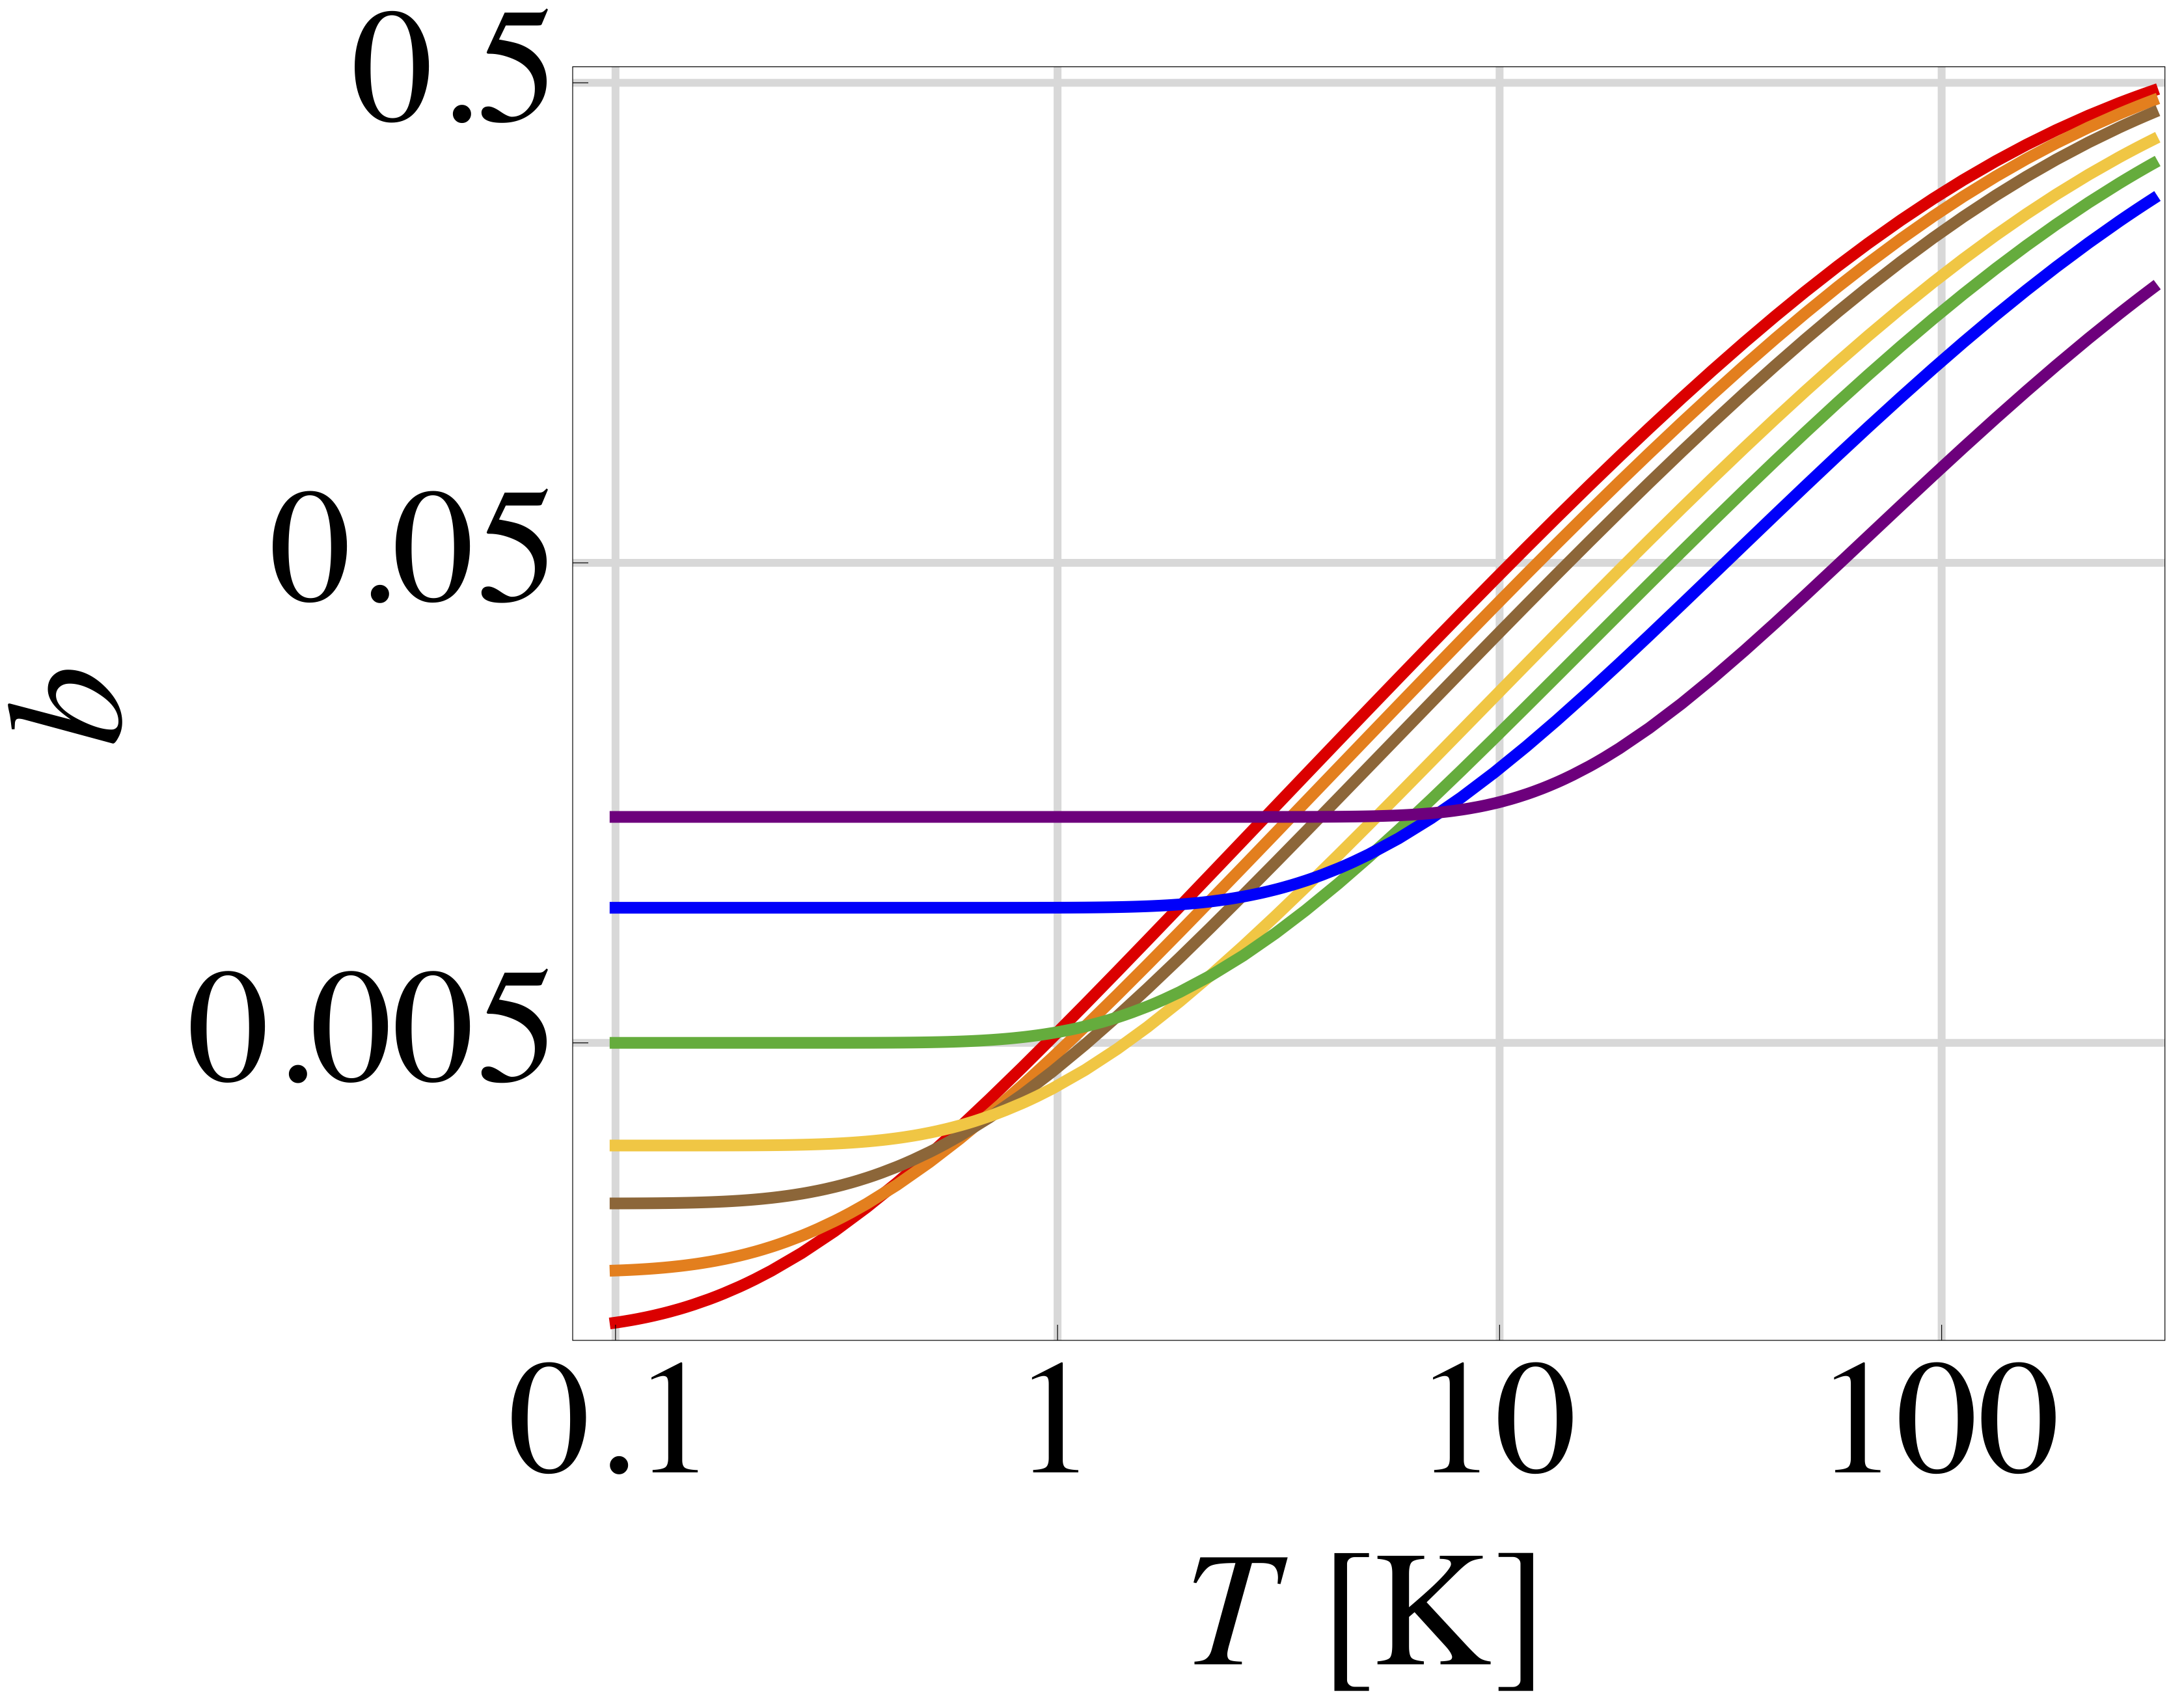
\includegraphics[width=3.8cm,height=3.3cm]{bloglog.png}
  \subcaption{\iffalse$N^*_T$ vs $T$\fi}
  \label{fig:cthcal2_4}
  %
\end{minipage}%
\vspace*{1.9cm}
\begin{minipage}[c][6cm][b]{.46\textwidth}
  \centering
  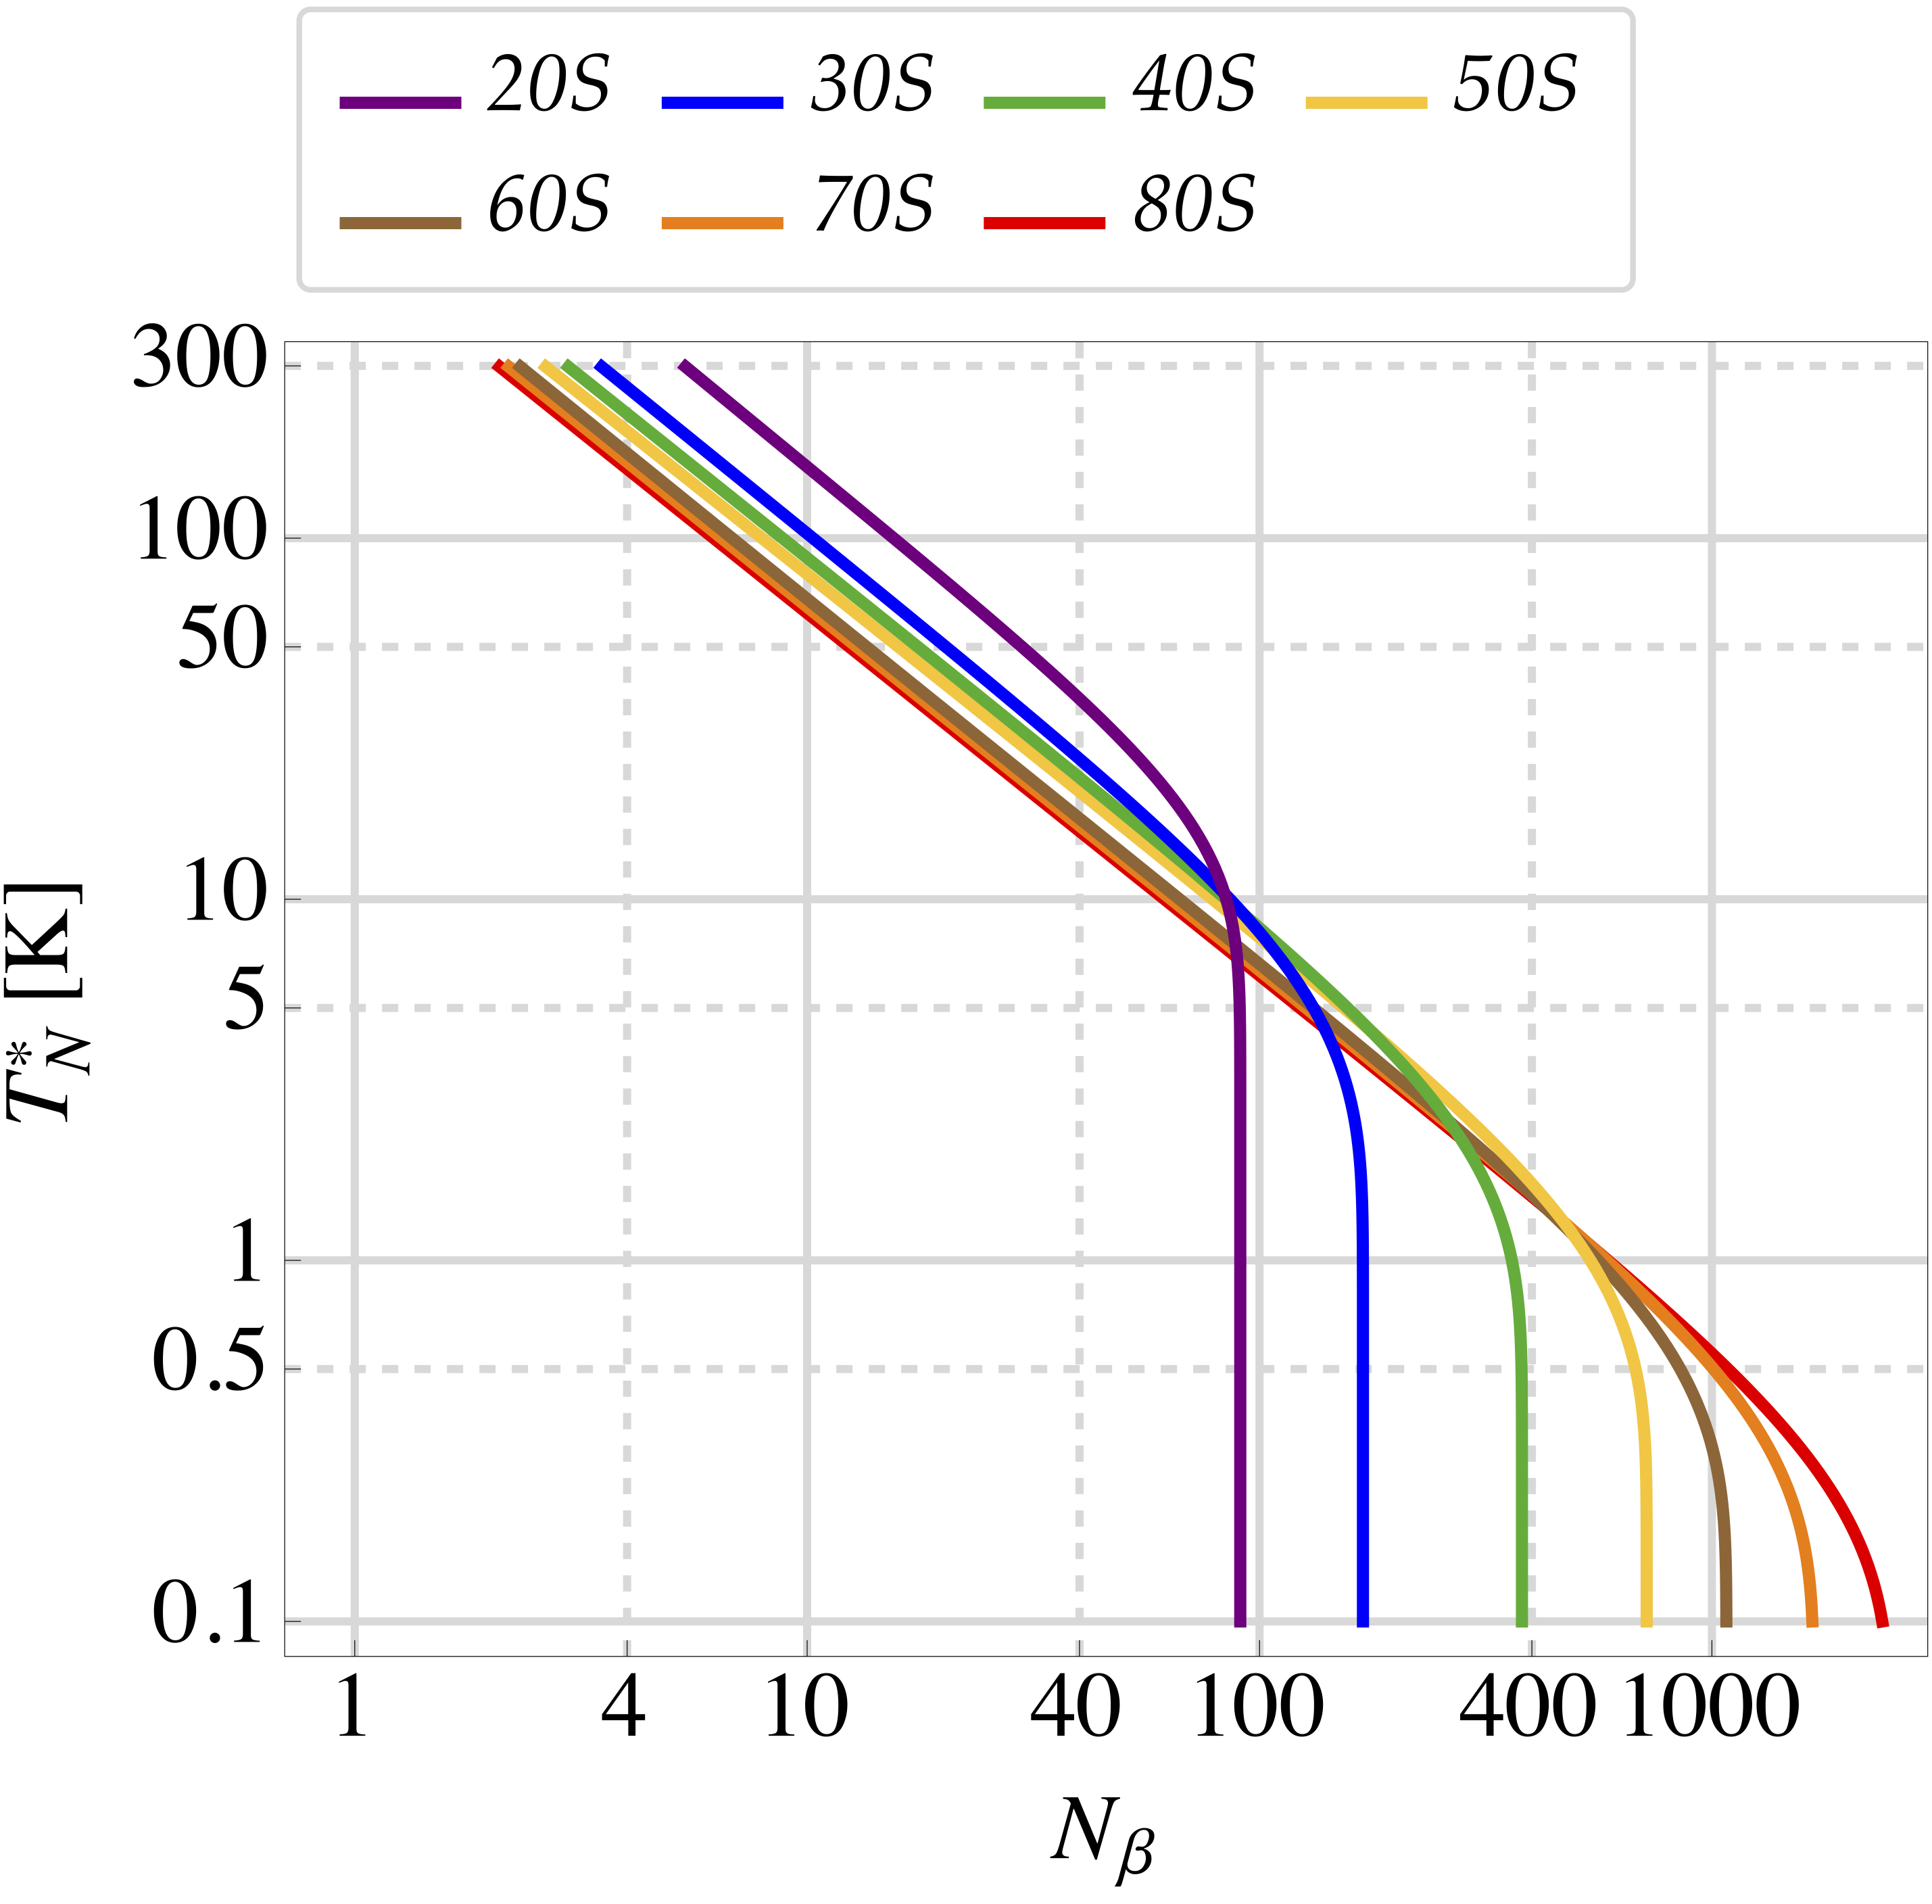
\includegraphics[width=7.0cm,height=6.8cm]{TvsNbloglog.png}
  \subcaption{\iffalse$N^*_T$ vs $T$\fi}
  \label{fig:cthcal3_4}
\end{minipage}
\caption{\textbf{$\bm{T^*_N}$, and the temperature  scaling of $\bm{b}$ and $\bm{\tau_0}$.} (a) Effective lifetime $\tau_0$ (determined by spontaneous emission and blackbody radiation-induced transitions) for different $nS$ $^{87}$Rb Rydberg states as a function of the ambient temperature. (b) Temperature dependence of the sum of branching ratios $b$ from the different $nS$ states to the contaminant $nP$ states playing a more relevant role in the avalanche dephasing process. (c)  Temperature $T^*_N$ needed to compensate for the dephasing effect as a function of $N_{\beta}$.}\label{fig:cthcal_4}
\end{figure}

Some Rydberg-dressing proposals \cite{pupillo2010}, \cite{Glaetzle2012}, \cite{Bouchoule2002}, \cite{Glaetzle2014} and previous experimental setups \cite{Bloch} making use of samples with an \textit{effective} $N_{\beta}\sim$ 30-70 would need an ambient temperature just above 10 K to make up for the dephasing effect. Such ambient temperatures are attainable using He dilution refrigerators \cite{CryoHeDiluRef1}, or by trapping the atoms close to a superconducting ring\cite{CryoSupercRing1}. The detrimental effects on those systems with an even lower atom number $N\sim 10$ \cite{vanBijnen2015}, \cite{Lee2013a} should become negligible for cryogenic temperatures around 70 K, which can be obtained using a Stirling refrigerator \cite{CryoStirlingRefrig}.

For several proposals where the atom number $N_0$ is $\gtrsim 100$ \cite{honer10a},\cite{maucher2011},\cite{Davis2016}, the van der Waals blockade radius $r_{\text{vdW}}$ is larger than or comparable to the sample dimensions. These will not be considerably affected by this dephasing process even if not working in a cryogenic environment. On the other hand, completely neutralizing the dephasing effect in proposals that rely on samples with $N_\beta \gtrsim 10^4$ (but with $r_{\text{vdW}}$ comparable to the interparticle spacing) as the one used in \cite{AB}, does not seem feasible by going to lower temperatures, as seen on Figure \ref{fig:cthcal_4}. \textcolor{Salmon}{(I haven't found a proposal explicitly requiring these conditions.)}

\begin{thebibliography}{8}
\bibitem{AB} 
E. A. Goldschmidt, T. Boulier, R. C. Brown, S. Koller, J. T. Young, A. V. Gorshkov, S. L. Rolston, and J. V. Porto, Phys. Rev. Lett. 116, 113001 (2016). \textcolor{ForestGreen}{Cited already in draft.}
 
\bibitem{Beterov2009} 
I. I. Beterov, I. I. Ryabtsev, D. B. Tretyakov, and V. M. Entin,
Phys. Rev. A 79, 052504 (2009). \textcolor{RedOrange}{Was not cited in draft.}


\bibitem{Dyachkov1994}
L. G. Dyachkov and P. M. Pankratov, J. Phys. B 27, 461
(1994). \textcolor{RedOrange}{Was not cited in draft.}


\bibitem{pupillo2010} G. Pupillo, A. Micheli, M. Boninsegni, I. Lesanovsky, and
P. Zoller, Phys. Rev. Lett. 104, 223002 (2010). \textcolor{ForestGreen}{Cited already in draft.}

\bibitem{honer10a} J. Honer, H. Weimer, T. Pfau, and H. P. B\"uchler, Phys. Rev. Lett. 105, 160404 (2010). \textcolor{ForestGreen}{Cited already in draft.}

\bibitem{Glaetzle2012} A. W. Glaetzle, R. Nath, B. Zhao, G. Pupillo, and P. Zoller, Physical Review A 86, 043403 (2012). \textcolor{ForestGreen}{Cited already in draft.}

\bibitem{vanBijnen2015} R. M. W. van Bijnen and T. Pohl, Phys. Rev. Lett. 114,
243002 (2015). \textcolor{ForestGreen}{Cited already in draft.}

\bibitem{Bouchoule2002} I. Bouchoule and K. M{\o}lmer, Phys. Rev. A 65, 041803
(2002). \textcolor{ForestGreen}{Cited already in draft.}

\bibitem{Lee2013a} T. E. Lee, S. Gopalakrishnan, and M. D. Lukin, Phys. Rev.
Lett. 110, 257204 (2013). \textcolor{ForestGreen}{Cited already in draft.}

\bibitem{Glaetzle2014}  A. W. Glaetzle, M. Dalmonte, R. Nath, I. Rousochatzakis,
R. Moessner, and P. Zoller, Phys. Rev. X 4, 041037 (2014). \textcolor{ForestGreen}{Cited already in draft.}

\bibitem{Bloch} J. Zeiher, R. van Bijnen, P. Schauß, S. Hild, J.-y. Choi, T. Pohl, I. Bloch, and C. Gross, Nature Physics (2016). \textcolor{ForestGreen}{Cited already in draft.}

\bibitem{maucher2011} F. Maucher, N. Henkel, M. Saffman, W. Krolikowski, S. Skupin, ´
and T. Pohl, Phys. Rev. Lett. 106, 170401 (2011). \textcolor{RedOrange}{Was not cited in draft.}

\bibitem{Davis2016} E. Davis, G. Bentsen, and M. Schleier-Smith, Approaching
the Heisenberg Limit without Single-Particle Detection,
Phys. Rev. Lett. 116, 053601 (2016). \textcolor{RedOrange}{Was not cited in draft.}

\bibitem{CryoHeDiluRef1} F. Jessen, M. Knufinke, S. Bell, P. Vergien, H. Hattermann, P. Weiss, M. Rudolph, M. Reinschmidt, K. Meyer, T. Gaber, D. Cano, A. G\"unther, S. Bernon, D. Koelle, R. Kleiner, and J. Fort\'agh, Appl. Phys. B 116, 665 (2014) \textcolor{RedOrange}{Was not cited in draft. Didn't read thoroughly. They claim $<$ 1 K ambient temperature for ultracold atomic clouds. Not sure if that's true. Interesting to read. Cited by other PRA's and PRL's.}

\bibitem{CryoSupercRing1}  P. Weiss, M. Knufinke, S. Bernon, D. Bothner, L. Sarkany, C. Zimmermann, R. Kleiner, D. Koelle, J. Fortagh, and H. Hattermann, Phys. Rev. Lett. 114, 113003 (2015).\textcolor{RedOrange}{Was not cited in draft.}

\bibitem{CryoStirlingRefrig} I. Ushijima, M. Takamoto, M. Das, T. Ohkubo, and H. Katori, Nat. Photonics 9, 185 (2015) \textcolor{RedOrange}{Was not cited in draft.}
\end{thebibliography}

\subparagraph{Comments on proposals.}

\begin{itemize}
\item \textbf{\cite{pupillo2010}} \textcolor{Cyan}{``In the following we provide example results for $N$=\textbf{13} atoms which we found to display all general features of mesoscopic cluster with $N\lesssim$ \textcolor{Magenta}{\textbf{40}}.''}
\item \textbf{\cite{honer10a}} \textcolor{Cyan}{``$\xi_0\equiv\left(C_6/2\hbar\left|\Delta\right|\right)^{1/6}$''}, column 1 of page 2. \textcolor{Cyan}{``$\xi_0=$ 3 $\mu$m''}, column 1 of page 4. Figure 3 shows the radius of the \textcolor{Magenta}{$N=10^5$} BEC is around 8 $\mu$m. $\Longrightarrow$ $r_{\text{vdW}}$ is \textcolor{Magenta}{\textbf{comparable}} to BEC size.

\item \textbf{\cite{Glaetzle2012}} \textcolor{Cyan}{``In this section we numerically investigate the effects of SE and BBR on the long-time dynamics of an ensemble of interacting Rydberg atoms by performing semiclassical molecular dynamics simulations.\ldots Using semiclassical molecular dynamics simulations we
study the resulting nonequilibrium dynamics of an ensemble
constitution of $N$ = \textcolor{Magenta}{\textbf{67}} Rydberg-dressed $^{85}$Rb atoms.''} Page 15.

\item \textbf{\cite{vanBijnen2015}} \textcolor{Cyan}{``As shown in Fig. 6(b) for $N$=\textcolor{Magenta}{\textbf{12}} atoms, adiabaticity can be achieved for \ldots As shown in Figs. 6(c) and 6(d), the dynamically prepared many-body state indeed exhibits this behavior to an extent\ldots''}. Page 4

\item \textbf{\cite{Bouchoule2002}} \textcolor{Cyan}{``Figure 3 shows the calculated evolution
of \textcolor{Magenta}{\textbf{20}} atoms illuminated by six lasers with appropriate relative
phases.''} Page 3.

\item \textbf{\cite{Lee2013a}} \textcolor{Cyan}{``Fig 4. Correlation function $\langle\sigma_m^x\sigma_n^x\rangle$ for 1D chain of \textcolor{Magenta}{\textbf{16}} spins, from simulating the master equation.} Page 4. \textcolor{Cyan}{``The gap was calculated using exact diagonalization for a 1D chain of \textcolor{Magenta}{\textbf{6}} spins with nearest-neighbor interactions.''} Supplemental material, page 3. Honestly, for this paper I'm not sure if the low atom number is just for simulation purposes or if that's the actual atom number they propose for real experiments.

\item \textbf{\cite{Glaetzle2014}} \textcolor{Cyan}{``In our exact diagonalizations (ED), we have considered finite-size clusters with periodic boundary conditions and $N$ =\textcolor{Magenta}{\textbf{16, 32, 36, 64, and 72}} sites.''} Page 12.

\item \textbf{\cite{Bloch}} \textcolor{Cyan}{``\ldots In this single $x$-$y$ plane, we then switched on a square optical lattice with $a_{\text{lat}}=$532 nm spacing and prepared about \textcolor{Magenta}{190} atoms in a unity filling Mott \ldots''}. You would claim $N\approx 200$ but since \textit{van der Waals} blockade radius $R_c=2\times a_{\text{latt}}$ (see figure 1) the actual $N$ is $N\approx 200/5 =$ \textcolor{Magenta}{\textbf{40}}.

\item \textbf{\cite{maucher2011}} They claim \textcolor{Magenta}{``N=100 atoms''} at the end of page 3. But \textcolor{Cyan}{``$R_{\text{vdW}} \approx$ 3 $\mu$m, \ldots''} page 4 and figure 3. Self-trapped condensate radius is around 3 $\mu$m, see Fig. 5. $\Longrightarrow$ $r_{\text{vdW}}$ is \textcolor{Magenta}{\textbf{comparable}} to BEC size.

\item \textbf{\cite{Davis2016}} \textcolor{Cyan}{``At a Rydberg-state population $\epsilon=0.1$, the ideal phase sensitivity of Eq. 5 can then be reached with up to $N_{\text{cr}}\approx$ \textcolor{Magenta}{150} atoms''} Page 4. However: \textcolor{Cyan}{``The coupling to $|R\rangle$ induces a two-body potential $V(r)$ that is nearly constant over a distance $L=\frac{1}{2}\left[C_6/\left(2\delta_{\text{R}}\right)\right]$ (Fig. 3b)''}, page 4. $\Longrightarrow$ $r_{\text{vdW}}$ is \textcolor{Magenta}{\textbf{comparable}} to sample size.
\end{itemize}

\end{document}